\documentclass[12pt,a4paper]{report}

\usepackage[a4paper,margin=1in]{geometry}
\usepackage{xcolor}
\usepackage{graphicx}
\usepackage{setspace}

\onehalfspacing

\begin{document}

%--------------------------------------------------
% COVER PAGE
%--------------------------------------------------

\begin{titlepage}
\centering

{\color{blue}\Huge\textbf{AKSHAR AI LTD}}\\[1cm]

{\color{black}\rule{12cm}{1pt}}\\[1.5cm]

{\LARGE\textbf{SUMMER INTERNSHIP PROJECT REPORT}}\\[1cm]

{\color{black}\rule{12cm}{1pt}}\\[1.5cm]

{\color{red}\Huge\textbf{AI/ML Model Performance}}\\[0.3cm]
{\color{red}\Huge\textbf{Benchmarking Tracker}}\\[2cm]

Submitted by\\[0.5cm]

{\Large\textbf{Shanvi Sinha}}\\
Enrollment No. 24162581051\\[1.5cm]

Guided By\\[0.5cm]

{\Large\textbf{Mr. Lokesh Budhia}}\\[2cm]

{\color{blue}In partial fulfillment for the award of the degree of}\\Bachelor of Technology in\\
Computer Science and Engineering\\[1cm]

\vfill

Ganpat University\\[1cm]



\end{titlepage}

%--------------------------------------------------
% CERTIFICATE
%--------------------------------------------------



\begin{center}
{\Large\textbf{CERTIFICATE}}
\end{center}

\vspace{1cm}

This is to certify that the Summer Internship Project work entitled \textbf{``AI/ML Model Performance Benchmarking Tracker''} carried out by \textbf{Shanvi Sinha} Enrollment No. \textbf{24162581051} a student of \textbf{Bachelor of Technology in Computer Science and Engineering} at \textbf{Ganpat University}, is a bonafide work completed during the internship \textbf{Akshar AI Ltd.}  under the guidance and supervision of \textbf{Mr. Lokesh Budhia} and \textbf{Mr. Hitendrasinh Rathod}.

The work presented in this report is original and has been completed as a part of the Summer Internship Program. To the best of our knowledge the project has not been submitted either in part or in full to any University or Institute for the award of any degree, diploma or certificate.

\vspace{2cm}

\textbf{Internal Guide Name and Signature}

\vspace{1.5cm}

\rule{6cm}{0.4pt}

\vspace{2cm}

\textbf{Head Name and Signature}

\vspace{1.5cm}

\rule{6cm}{0.4pt}

\vspace{2cm}

\textbf{Place:}

\vspace{0.5cm}

\textbf{Date:} \rule{3cm}{0.4pt}

\newpage

\begin{center}
{\Large\textbf{DECLARATION}}
\end{center}

I hereby declare that the internship project entitled \textbf{``AI/ML Model Performance Benchmarking Tracker''} submitted in partial fulfillment of the requirements for the award of the degree of \textbf{Bachelor of Technology in Computer Science and Engineering} is my original work carried out during my internship at \textbf{Akshar AI Ltd.} under the guidance of \textbf{Mr. Lokesh Budhia} and \textbf{Mr. Hitendrasinh Rathod}.

I further declare that this project has not been submitted either in part or in full to any other university or institution for the award of any degree, diploma or certificate.

\vspace{2cm}

\begin{flushleft}
\textbf{Shanvi Sinha}\\
 24162581051
\end{flushleft}

\newpage


%--------------------------------------------------
% ACKNOWLEDGEMENT
%--------------------------------------------------

\begin{center}
\textbf{\Large ACKNOWLEDGEMENT}
\end{center}

\vspace{1cm}

Summer Internship project has provided me with an excellent opportunity for learning and self-development. I would like to express my sincere gratitude to my Internal Guide, \textbf{Mr. Lokesh Budhia} and my Industry Guide \textbf{Mr. Hitendrasinh Rathod} for their valuable guidance, encouragement and support throughout the project.

I am also thankful to the faculty members of Ganpat University for providing me with the opportunity and resources required for the successful completion of this internship project.

Finally, I would like to thank my family and friends for their constant motivation and support during this journey.

\vspace{1cm}

\begin{flushleft}
\textbf{SHANVI SINHA}\\
24162581051
\end{flushleft}

\newpage


\begin{center}
\textbf{\Large ABSTRACT}
\end{center}

\vspace{1cm}

Machine Learning models require high-quality data for accurate analysis and evaluation. This project \textbf{AI/ML Model Performance Benchmarking Tracker} focuses on data understanding, preprocessing and exploratory data analysis of a machine learning benchmark dataset.

Various techniques such as data cleaning, handling missing values, duplicate removal and data validation were performed to improve dataset quality. Exploratory Data Analysis (EDA) was carried out to identify patterns, trends and relationships within the data.

The project provides a structured and reliable dataset that can be used for future machine learning benchmarking and performance evaluation.

\newpage

\chapter*{CONTENTS}
\addcontentsline{toc}{chapter}{Contents}

Certificate \dotfill

Declaration \dotfill

Acknowledgement \dotfill

Abstract \dotfill

Contents \dotfill

List of Figures \dotfill

List of Tables \dotfill

\vspace{0.3cm}

\textbf{1: INTRODUCTION} \dotfill

1.1 Project Overview \dotfill

1.2 Background of the Study \dotfill

1.3 Problem Statement \dotfill

1.4 Project Objectives \dotfill

1.5 Scope of the Project \dotfill

1.6 Project Deliverables \dotfill

1.7 Report Organization \dotfill

\vspace{0.3cm}

\textbf{2: REQUIREMENT ANALYSIS} \dotfill

2.1 Domain Study \dotfill

2.2 Existing System Analysis \dotfill

2.3 Proposed System \dotfill

2.4 Functional Requirements \dotfill

2.5 Non-Functional Requirements \dotfill

2.6 Tools and Technologies Used \dotfill

\vspace{0.3cm}

\textbf{3: DATA COLLECTION AND UNDERSTANDING} \dotfill

3.1 Data Source \dotfill

3.2 Data Description \dotfill

3.3 Data Structure \dotfill

3.4 Data Dictionary \dotfill

3.5 Data Quality Assessment \dotfill

\vspace{0.3cm}

\textbf{4: DATA PREPROCESSING} \dotfill

4.1 Data Cleaning \dotfill

4.2 Handling Missing Values \dotfill

4.3 Duplicate Removal \dotfill

4.4 Data Transformation \dotfill

4.5 Data Validation \dotfill

4.6 Final Prepared Dataset \dotfill

\vspace{0.3cm}

\textbf{5: DATA ANALYSIS AND MODELING} \dotfill

5.1 Exploratory Data Analysis (EDA) \dotfill

5.2 Data Relationships \dotfill

5.3 Key Metrics Identification \dotfill

\newpage

\chapter*{\color{ChapterBlue}1 INTRODUCTION}

\setcounter{chapter}{1}
\setcounter{section}{0}

\section{Project Overview}

Artificial Intelligence (AI) and Machine Learning (ML) have become important technologies for solving real-world problems and supporting data-driven decision making. The performance of machine learning models depends not only on the algorithms used but also on the quality of data and evaluation methods applied during analysis.

The \textbf{AI/ML Model Performance Benchmarking Tracker} project focuses on understanding, preprocessing, and analyzing benchmark datasets used in machine learning applications. The project aims to establish a structured workflow for data preparation and exploratory analysis so that reliable benchmarking and model evaluation can be performed in the future. Through systematic data analysis, important patterns, trends, and insights can be identified, helping researchers and developers make informed decisions regarding model performance.

\section{Background of the Study}

Machine Learning models are widely used in various domains such as healthcare, finance, education, retail, and business analytics. As the number of available machine learning algorithms continues to grow, comparing their performance has become an important task. Different models may produce different results depending on the dataset, preprocessing techniques, and evaluation criteria used.

Benchmarking is the process of evaluating and comparing models using standardized datasets and performance metrics. Reliable benchmarking requires clean, accurate, and well-structured data. Poor data quality can lead to inaccurate predictions and misleading conclusions. Therefore, data preprocessing and exploratory analysis play a significant role in improving the reliability of machine learning experiments.

This project focuses on dataset preparation and analysis, which serve as the foundation for future benchmarking and model performance evaluation activities.

\section{Problem Statement}

Machine learning datasets often contain missing values, duplicate records, inconsistent formats, and other data quality issues. These problems can negatively affect analysis results and reduce the effectiveness of machine learning models.

In addition, comparing machine learning models without a structured benchmarking process may lead to unreliable conclusions. The absence of proper data preparation and analysis makes it difficult to identify the strengths and weaknesses of different models.

Therefore, there is a need for a systematic approach that focuses on data understanding, preprocessing, exploratory analysis, and metric identification. This project addresses these challenges by preparing a clean and reliable dataset suitable for future benchmarking and performance evaluation.

\section{Project Objectives}

The main objectives of this project are:

\begin{itemize}
\item To understand the structure and characteristics of the benchmark dataset.
\item To perform data cleaning and preprocessing operations.
\item To identify and handle missing values and duplicate records.
\item To conduct Exploratory Data Analysis (EDA) using statistical and graphical techniques.
\item To discover patterns and relationships within the dataset.
\item To identify key metrics useful for AI/ML benchmarking.
\item To prepare a reliable dataset for future model evaluation.
\item To document the complete workflow and findings of the project.
\end{itemize}

\section{Scope of the Project}

The scope of this project is limited to data collection, understanding, preprocessing, and exploratory analysis of a benchmark dataset. The project focuses on improving data quality and generating meaningful insights through various analytical techniques.

Activities such as data cleaning, missing value handling, duplicate removal, data validation, and visualization are included within the project scope. The project does not involve the deployment of machine learning models but provides a strong foundation for future benchmarking and performance evaluation studies.

\section{Project Deliverables}

The following deliverables were produced during the project:

\begin{itemize}
\item Cleaned and validated benchmark dataset.
\item Data preprocessing notebook developed using Google Colab.
\item Exploratory Data Analysis (EDA) results and visualizations.
\item Statistical summaries and analytical findings.
\item Identification of key benchmarking metrics and indicators.
\item GitHub repository containing project files and documentation.
\item Final internship project report.
\end{itemize}

\section{Report Organization}

This report is organized into multiple chapters, each describing a specific phase of the project. Chapter 1 introduces the project, including its objectives, scope, and problem statement. Chapter 2 presents the requirement analysis, domain study, and technologies used during development.

Chapter 3 focuses on data collection and understanding, including dataset description, structure, and quality assessment. Chapter 4 explains the preprocessing techniques applied to improve data quality and prepare the dataset for analysis.

Chapter 5 presents the Exploratory Data Analysis (EDA), data relationships, and key metrics identified during the study. Together, these chapters provide a comprehensive overview of the project and its outcomes.

\chapter*{\color{ChapterBlue}2 REQUIREMENT ANALYSIS}
\addcontentsline{toc}{chapter}{2: REQUIREMENT ANALYSIS}

\setcounter{chapter}{2}
\setcounter{section}{0}
\renewcommand{\thesection}{2.\arabic{section}}

\section{Domain Study}

Artificial Intelligence (AI) and Machine Learning (ML) have become essential technologies in modern data-driven applications. Organizations use machine learning models to analyze data, identify patterns and make predictions that support decision-making processes. As the number of available machine learning algorithms continues to increase evaluating their performance accurately has become an important task.

Benchmarking provides a systematic way to compare models using standard datasets and evaluation metrics. A well-structured benchmarking process helps researchers and developers select the most suitable model for a particular problem while ensuring reliability and consistency in results.

\section{Existing System Analysis}

Many machine learning projects focus primarily on model development and often overlook the importance of data quality assessment. Datasets may contain missing values, duplicate records, inconsistent formats and irrelevant information which can negatively impact model performance.

Existing approaches may not provide a standardized workflow for dataset preparation and analysis. As a result, model evaluation and comparison may produce unreliable outcomes making it difficult to draw accurate conclusions regarding model effectiveness.

\section{Proposed System}

The proposed system focuses on creating a structured framework for dataset preparation and analysis before model benchmarking. The system includes data collection, data understanding, preprocessing, validation and exploratory data analysis.

The objective is to ensure that datasets are clean, consistent and reliable before being used for benchmarking purposes. This approach improves the quality of analysis and provides a strong foundation for future machine learning model evaluation.

\section{Functional Requirements}

The system should perform the following functions:

\begin{itemize}
\item Load and analyze benchmark datasets.
\item Identify missing values and data inconsistencies.
\item Remove duplicate records.
\item Perform data cleaning and preprocessing.
\item Generate statistical summaries.
\item Create visualizations for exploratory analysis.
\item Identify important benchmarking metrics.
\item Document analytical findings and results.
\end{itemize}

\section{Non-Functional Requirements}

The system should satisfy the following non-functional requirements:

\begin{itemize}
\item Accuracy in data processing and analysis.
\item Reliability of generated outputs.
\item Scalability for handling larger datasets.
\item Maintainability of code and documentation.
\item Efficiency in data processing operations.
\item Reproducibility of analysis results.
\item Usability through a clear and organized workflow.
\end{itemize}

\section{Tools and Technologies Used}

The following tools and technologies were used during the project:

\begin{itemize}
\item \textbf{Python} for data analysis and preprocessing.
\item \textbf{Google Colab} as the development environment.
\item \textbf{Pandas} for data manipulation and cleaning.
\item \textbf{NumPy} for numerical computations.
\item \textbf{Matplotlib} for data visualization.
\item \textbf{Git} for version control.
\item \textbf{GitHub} for repository management and collaboration.
\item \textbf{NotebookLM} for documentation support.
\item \textbf{Overleaf} for preparing the final internship report.
\end{itemize}

\addcontentsline{toc}{chapter}{3 DATA COLLECTION AND UNDERSTANDING}

\setcounter{chapter}{3}
\setcounter{section}{0}
\renewcommand{\thesection}{3.\arabic{section}}

\chapter*{\color{ChapterBlue}3 DATA COLLECTION AND UNDERSTANDING}
\section{Data Source}

The dataset used in this project was obtained from publicly available benchmark sources commonly used for machine learning and data analysis tasks. The dataset was selected because it contains multiple attributes suitable for preprocessing, analysis, and future benchmarking activities.

The data was imported into Google Colab for further examination and processing. The dataset serves as the foundation for understanding data quality issues and performing analytical tasks required for machine learning workflows.
\vspace{0.5cm}
\begin{figure}
    \centering
    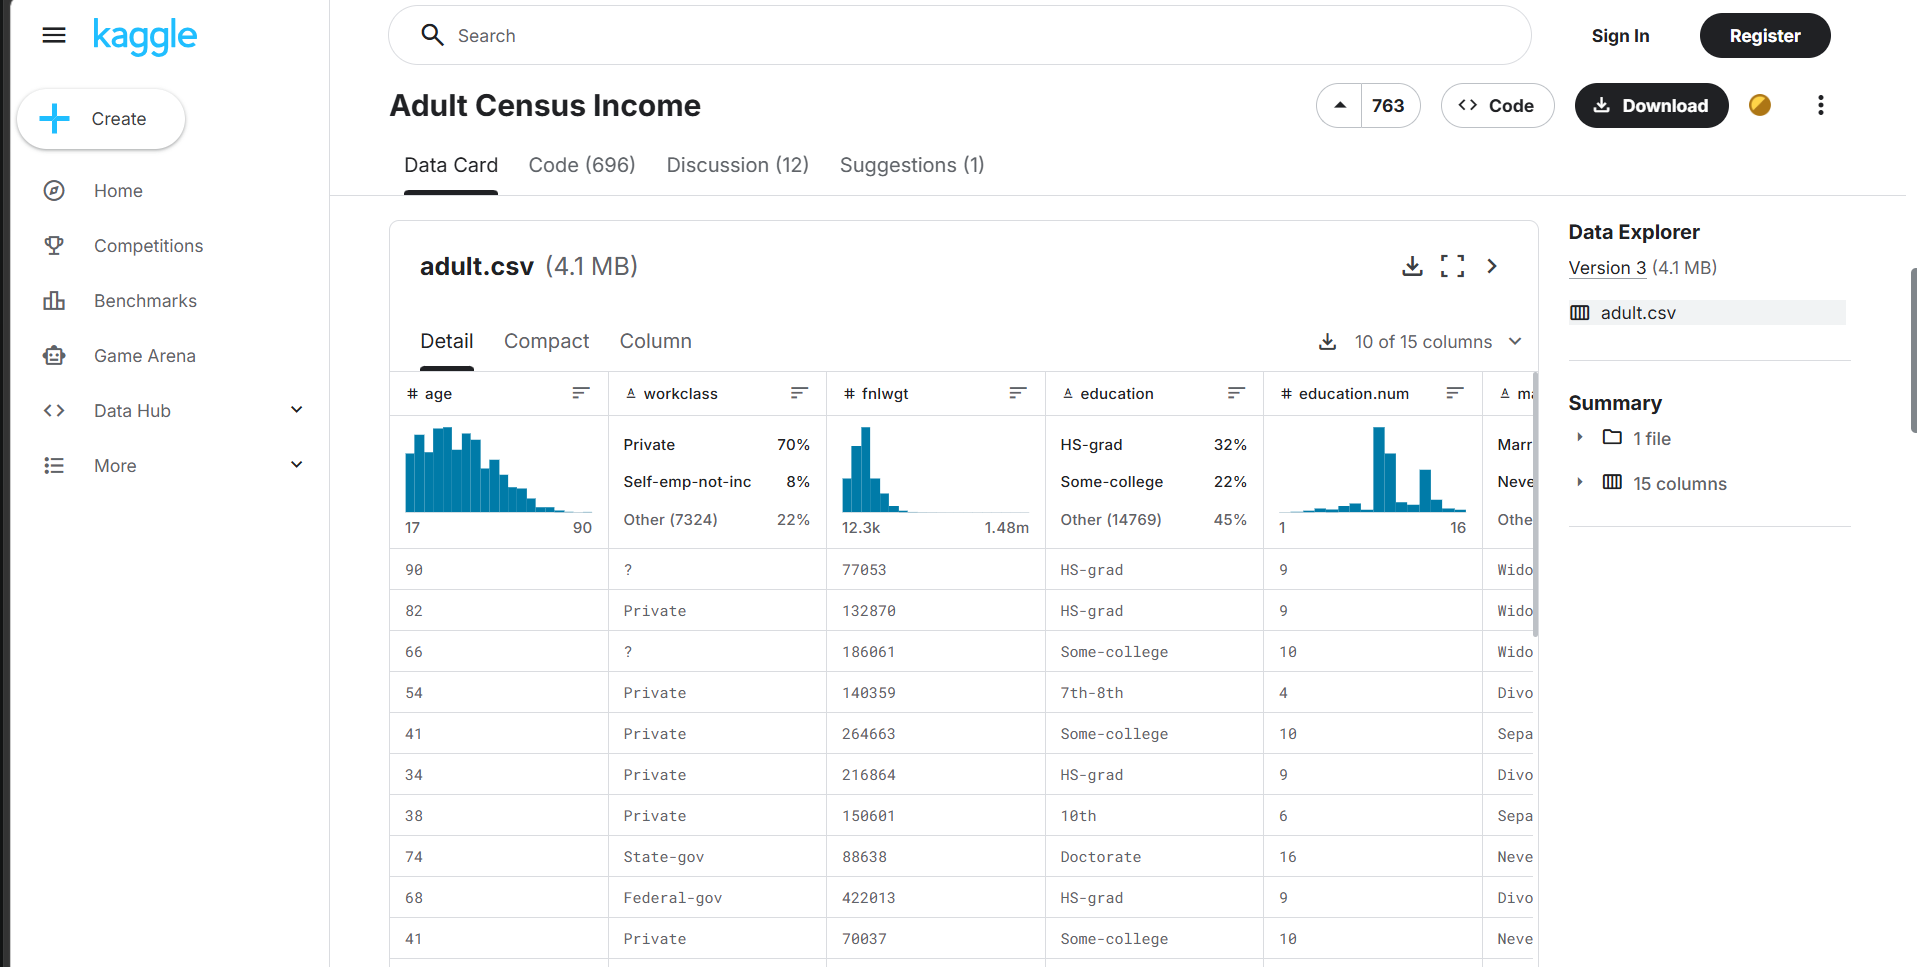
\includegraphics[width=0.75\linewidth]{kaggle_3_1.png}
    \caption{Adult Census Income Dataset from Kaggle}
    \label{fig:Dataset_source}
\end{figure}
\newpage
\vspace{1cm}


\section{Data Description}

The dataset used in this project contains demographic, educational, and employment-related information collected from individuals. The primary objective of the dataset is to support machine learning and data analysis tasks by providing various attributes that can be used for classification and prediction purposes.

The dataset consists of both numerical and categorical features. Numerical attributes represent measurable values, while categorical attributes describe different categories and groups. These attributes provide valuable information that can be analyzed to identify patterns, relationships, and trends within the data.

The dataset contains multiple records, where each row represents an individual observation and each column represents a specific feature. Understanding the characteristics of the dataset is important before performing preprocessing and analytical operations.

Table 3.1 provides a summary of the dataset.
\begin{center}
\small
\textbf{Table 3.1: Dataset Summary}

\vspace{0.2cm}

\begin{tabular}{|p{4cm}|p{6cm}|}
\hline
\textbf{Property} & \textbf{Value} \\
\hline
Dataset Name & Adult Census Income Dataset \\
\hline
Source & Kaggle \\
\hline
Number of Records & 48,842 \\
\hline
Number of Attributes & 15 \\
\hline
Data Type & Mixed (Numerical and Categorical) \\
\hline
Target Variable & Income \\
\hline
\end{tabular}
\end{center}
\vspace{0.2cm}

The first five records of the dataset are shown in Figure 3.2. These records provide an overview of the dataset structure and the values contained in different attributes.
\begin{center}
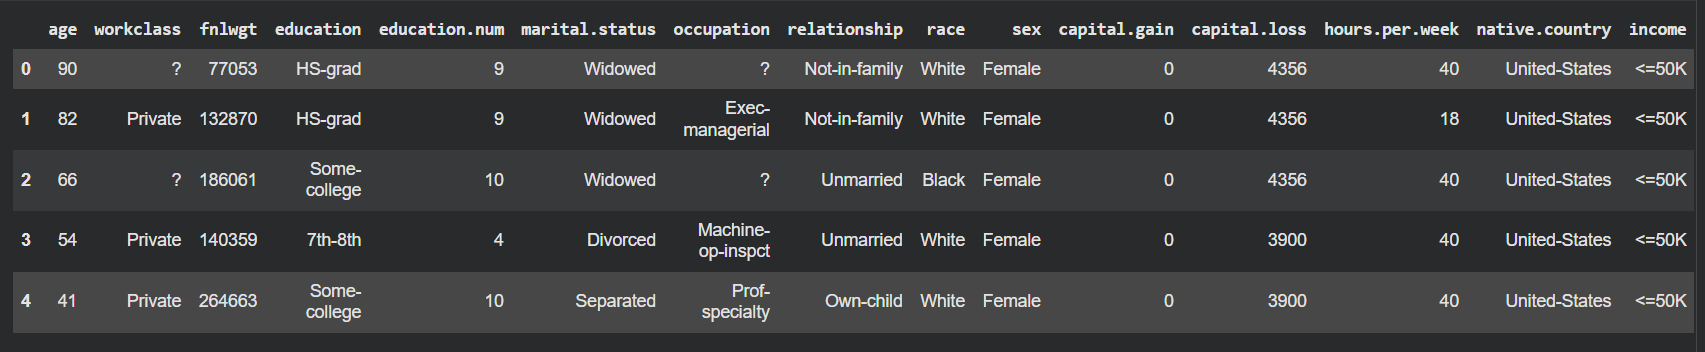
\includegraphics[width=0.65\textwidth]{DFHEAD_3_2.PNG}

\vspace{0.2cm}

\textbf{Figure 3.2: First Five Records of the Dataset}
\end{center}
\vspace{1cm}
\section{Data Structure}

Understanding the structure of the dataset is an important step before performing data preprocessing and analysis. The dataset structure provides information about the number of records, attributes, and data types present in the dataset.

The Adult Census Income dataset contains a combination of numerical and categorical attributes. Each row represents an individual record, while each column represents a specific feature related to demographic, educational, and employment information.

To understand the dataset structure, functions such as \texttt{df.shape()}, \texttt{df.info()}, and \texttt{df.columns} were used. These functions helped identify the dimensions of the dataset, available attributes, and their respective data types.

Table 3.2 summarizes the overall structure of the dataset.

\begin{center}
\small
\textbf{Table 3.2: Dataset Structure Summary}

\vspace{0.2cm}

\begin{tabular}{|p{5cm}|p{5cm}|}
\hline
\textbf{Property} & \textbf{Value} \\
\hline
Total Records & 48,842 \\
\hline
Total Attributes & 15 \\
\hline
Numerical Features & 6 \\
\hline
Categorical Features & 9 \\
\hline
Target Variable & Income \\
\hline
\end{tabular}
\end{center}

The dimensions of the dataset are shown in Figure 3.3.

\begin{center}
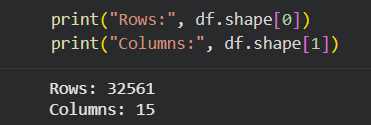
\includegraphics[width=0.6\textwidth]{3_3_Dataset Dimensions.png}

\vspace{0.2cm}

\textbf{Figure 3.3: Dataset Dimensions}
\end{center}
\vspace{1cm}
\section{Data Dictionary}

A data dictionary provides detailed information about each attribute present in the dataset. It helps in understanding the meaning, purpose, and type of data stored in each column. The Adult Census Income dataset contains demographic, educational, and employment-related attributes that are useful for machine learning and data analysis tasks.

Table~3.3 presents the data dictionary of the dataset.


\vspace{1cm}
\begin{center}
\small
\textbf{Table 3.3: Data Dictionary}
\vspace{0.65cm}
\begin{tabular}{|p{3cm}|p{8cm}|}
\hline
\textbf{Attribute} & \textbf{Description} \\
\hline
age & Age of the individual \\
\hline
workclass & Employment type of the individual \\
\hline
fnlwgt & Final sampling weight assigned by census bureau \\
\hline
education & Highest education level attained \\
\hline
education-num & Numerical representation of education level \\
\hline
marital-status & Marital status of the individual \\
\hline
occupation & Type of occupation or job role \\
\hline
relationship & Relationship status within the family \\
\hline
race & Race category of the individual \\
\hline
sex & Gender of the individual \\
\hline
capital-gain & Capital gains earned during the year \\
\hline
capital-loss & Capital losses incurred during the year \\
\hline
hours-per-week & Average working hours per week \\
\hline
native-country & Country of origin of the individual \\
\hline
income & Income category (Target Variable) \\
\hline
\end{tabular}
\end{center}
\vspace{1cm}

\section{Data Quality Assessment}

Data quality assessment is an important step in the data preparation process. It helps identify issues such as missing values, duplicate records, incorrect data types, and inconsistencies that may affect the accuracy of analysis and machine learning models.

The Adult Census Income dataset was examined to evaluate its overall quality before performing preprocessing operations. Various checks were conducted to identify missing values, duplicate entries, and data completeness.

The assessment revealed that the dataset contained some missing values represented by special characters in categorical attributes. Duplicate records were also checked to ensure data consistency. These findings helped determine the preprocessing steps required to prepare a clean and reliable dataset for further analysis.
The results of the data quality assessment are presented below.
\vspace{1cm}
\begin{figure}
    \centering
    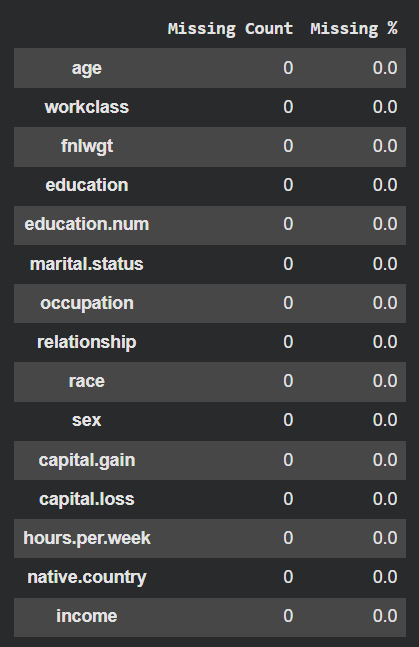
\includegraphics[width=0.5\linewidth]{missing_values_3_5.png}
    \caption{Missing Values Analysis}
    \label{Figure 3.4: Missing Values Analysis}
\end{figure}

 

\clearpage

\setcounter{chapter}{4}
\setcounter{section}{0}
\renewcommand{\thesection}{4.\arabic{section}}

\chapter*{\color{ChapterBlue}4:\ DATA PREPROCESSING}
\addcontentsline{toc}{chapter}{4: DATA PREPROCESSING}

%%%%%%%%%%%%%%%%%%%%%%%%%%%%%%%%%%%%%%%%%%%%%%%%%%
% 4.1 DATA CLEANING
%%%%%%%%%%%%%%%%%%%%%%%%%%%%%%%%%%%%%%%%%%%%%%%%%%

\section{Data Cleaning}

Data cleaning is a fundamental step in the data preprocessing process. Real-world datasets often contain inconsistencies, missing values, duplicate records, incorrect data formats, and other quality issues that can affect the accuracy of analysis and machine learning models.

In this project, the Adult Census Income dataset was carefully examined to identify potential data quality problems. The dataset was inspected for missing values, duplicate entries, inconsistent formatting, and incorrect data types. Appropriate cleaning techniques were applied to improve the overall quality and reliability of the data.

During the cleaning process, unnecessary inconsistencies were removed and the dataset was standardized to ensure uniformity across all attributes. These activities helped create a structured and reliable dataset suitable for further preprocessing and analytical tasks.

Data cleaning plays an important role in improving the effectiveness of machine learning workflows, as clean and accurate data leads to more reliable insights and better model performance. The cleaned dataset served as the foundation for the subsequent stages of preprocessing, analysis, and benchmarking.

%%%%%%%%%%%%%%%%%%%%%%%%%%%%%%%%%%%%%%%%%%%%%%%%%%
% 4.2 HANDLING MISSING VALUES
%%%%%%%%%%%%%%%%%%%%%%%%%%%%%%%%%%%%%%%%%%%%%%%%%%

\section{Handling Missing Values}

Missing values can negatively impact the quality of data analysis and machine learning models. Therefore, identifying and handling missing data is an essential preprocessing activity.

The dataset was examined to identify missing values present in different attributes. Appropriate methods were applied to handle missing entries and improve data completeness. This process reduced inconsistencies and enhanced the reliability of the dataset.

Figure 4.1 illustrates the missing value analysis performed during preprocessing.

\begin{center}
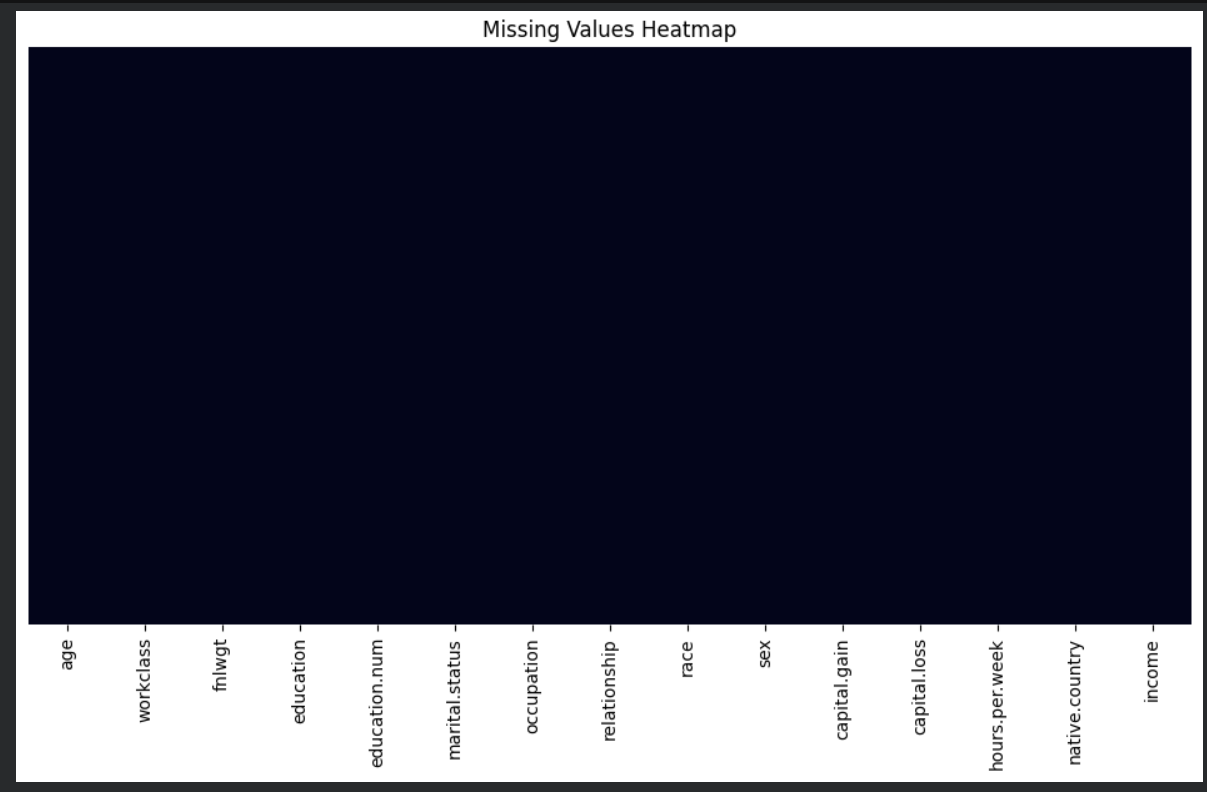
\includegraphics[width=0.75\textwidth]{missing_values_4_2.png}

\vspace{0.2cm}

\textbf{Figure 4.1: Missing Values Analysis}
\end{center}

%%%%%%%%%%%%%%%%%%%%%%%%%%%%%%%%%%%%%%%%%%%%%%%%%%
% 4.3 DUPLICATE REMOVAL
%%%%%%%%%%%%%%%%%%%%%%%%%%%%%%%%%%%%%%%%%%%%%%%%%%

\section{Duplicate Removal}

Duplicate records can introduce redundancy and affect the accuracy of analytical results. Therefore, the dataset was checked for duplicate entries during preprocessing.

Duplicate detection techniques were applied to identify repeated records. Any unnecessary duplicate entries were removed to ensure that each observation represented unique information. This improved the consistency and integrity of the dataset.

The removal of duplicate records contributed to the creation of a cleaner and more reliable dataset suitable for further analysis.

%%%%%%%%%%%%%%%%%%%%%%%%%%%%%%%%%%%%%%%%%%%%%%%%%%
% 4.4 DATA TRANSFORMATION
%%%%%%%%%%%%%%%%%%%%%%%%%%%%%%%%%%%%%%%%%%%%%%%%%%

\section{Data Transformation}

Data transformation involves converting data into a suitable format for analysis and machine learning applications. This step helps standardize the dataset and improve its usability.

Various transformations were performed on the dataset, including verification of data types and formatting of attributes. These transformations ensured that the dataset followed a consistent structure and could be processed efficiently during analysis.


%%%%%%%%%%%%%%%%%%%%%%%%%%%%%%%%%%%%%%%%%%%%%%%%%%
% 4.5 DATA VALIDATION
%%%%%%%%%%%%%%%%%%%%%%%%%%%%%%%%%%%%%%%%%%%%%%%%%%

\section{Data Validation}

Data validation was performed to verify the correctness, completeness, and consistency of the processed dataset. Validation checks were conducted after data cleaning and transformation activities.

The dataset was examined for missing values, duplicate records, invalid entries, and data type inconsistencies. The validation process confirmed that the dataset was properly prepared for exploratory analysis and future machine learning tasks.

Successful validation ensured that the final dataset met the quality standards required for reliable analytical operations.

%%%%%%%%%%%%%%%%%%%%%%%%%%%%%%%%%%%%%%%%%%%%%%%%%%
% 4.6 FINAL PREPARED DATASET
%%%%%%%%%%%%%%%%%%%%%%%%%%%%%%%%%%%%%%%%%%%%%%%%%%

\section{Final Prepared Dataset}

After completing all preprocessing activities, a clean and structured dataset was obtained. The final dataset was free from major quality issues and was prepared for exploratory data analysis and machine learning applications.

The preprocessing phase improved data quality by handling missing values, removing duplicate records, performing necessary transformations, and validating the results. The final prepared dataset serves as a reliable foundation for subsequent analytical tasks.

Figure 4.2 shows a sample of the final prepared dataset used for further analysis.

\begin{center}
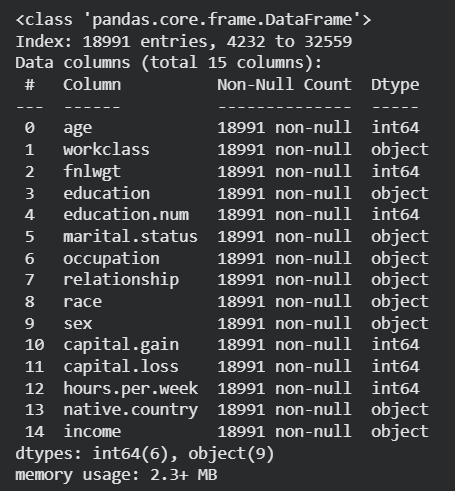
\includegraphics[width=0.85\textwidth]{final_dataset_4_6.png}

\vspace{0.2cm}

\textbf{Figure 4.2: Final Prepared Dataset}
\end{center}

\clearpage

\setcounter{chapter}{5}
\setcounter{section}{0}
\renewcommand{\thesection}{5.\arabic{section}}

\chapter*{\color{ChapterBlue}5\ DATA ANALYSIS AND MODELING}
\addcontentsline{toc}{chapter}{5 DATA ANALYSIS AND MODELING}
\section{Exploratory Data Analysis (EDA)}

Exploratory Data Analysis (EDA) is the process of examining and visualizing data to understand its characteristics, patterns, and trends. EDA helps identify relationships between variables, detect anomalies, and generate meaningful insights before applying machine learning techniques.

In this project, various statistical and graphical methods were used to analyze the Adult Census Income dataset. Different visualizations were created to understand the distribution of attributes and identify important trends within the data.

The analysis provided a deeper understanding of the dataset and supported the identification of key factors influencing income classification.

\begin{figure}
    \centering
    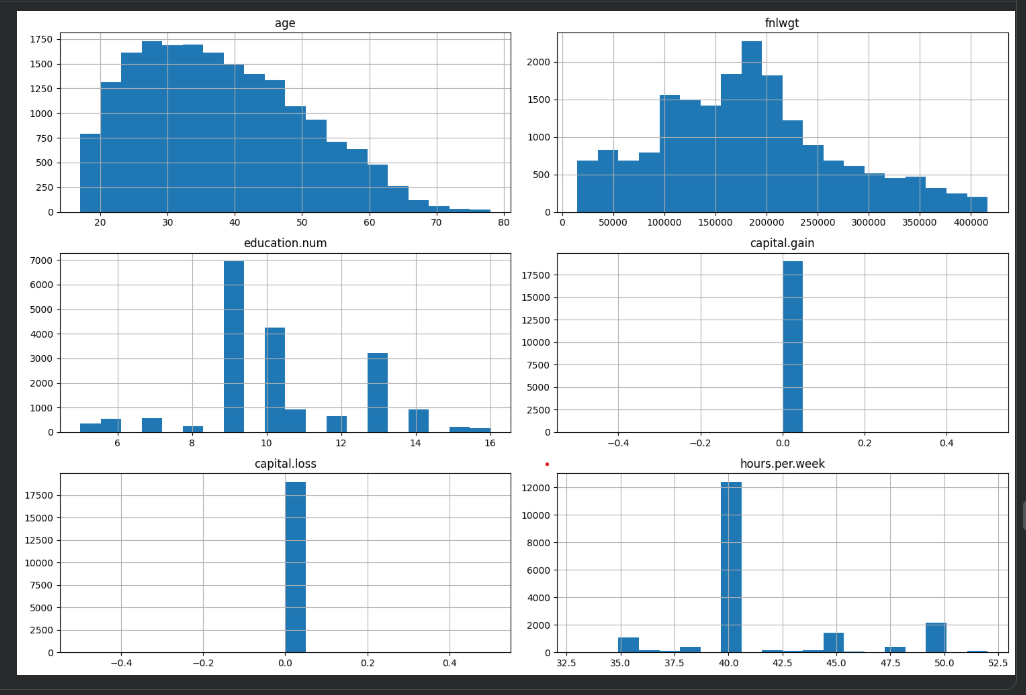
\includegraphics[width=0.5\linewidth]{eda_histogram_5_1.png}
    \caption{Distribution of Numerical Features}
    \label{fig:eda_histogram}
\end{figure}
\newpage
\section{Data Relationships}

Understanding the relationships between different variables is an important aspect of exploratory data analysis. Identifying these relationships helps determine how attributes influence one another and provides valuable insights for future machine learning model development.

In this project, correlation analysis was performed on the numerical attributes of the Adult Census Income dataset. A correlation heatmap was generated to visualize the strength and direction of relationships between variables.

The heatmap helps identify positive and negative correlations among features and highlights attributes that may have a significant impact on the target variable. Understanding these relationships supports better feature selection and improves the effectiveness of predictive modeling.
\begin{figure}
    \centering
    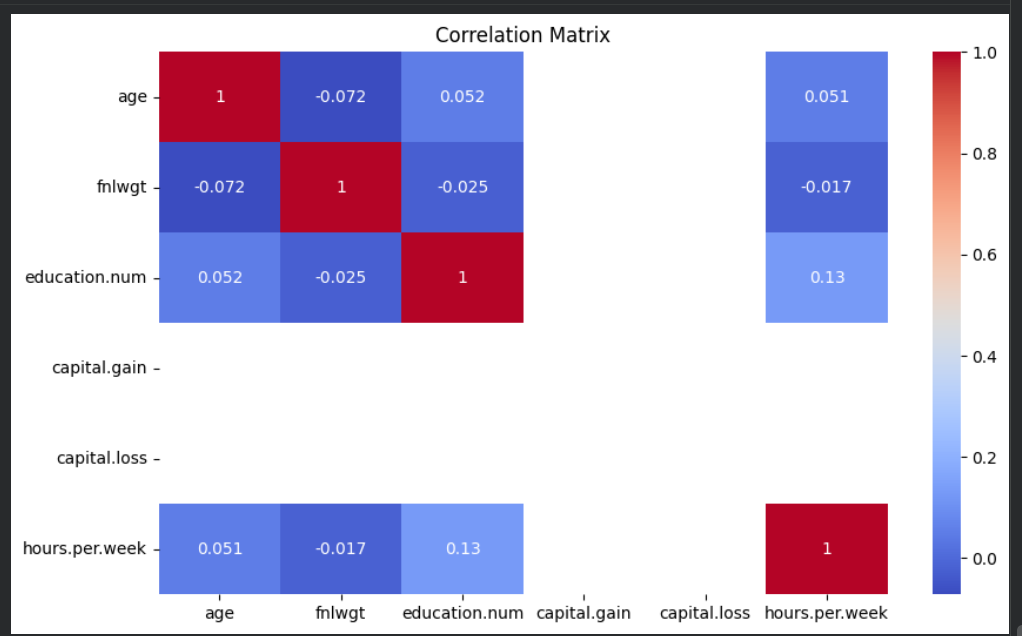
\includegraphics[width=0.5\linewidth]{correlation_heatmap_5_2.png}
    \caption{Correlation Heatmap of Numerical Features}
    \label{fig:correlation_heatmap}
\end{figure}

\section{Key Metrics Identification}

Identifying key metrics is an important part of data analysis and benchmarking. These metrics provide valuable information about the quality, structure, and characteristics of the dataset. They also help evaluate the readiness of the dataset for machine learning applications and future performance assessment activities.

During the analysis process, several important metrics were identified and examined. These metrics included the total number of records, number of attributes, missing values, duplicate records, data types, and target variable distribution. Understanding these metrics helped assess the overall quality and usability of the dataset.

The identified metrics serve as a foundation for future AI/ML benchmarking activities and support informed decision-making during model development and evaluation.

Table~\ref{tab:key_metrics} presents the key metrics identified during the analysis process.
\begin{table}[H]
\centering
\caption{Key Metrics Identified}
\label{tab:key_metrics}

\begin{tabular}{|p{5cm}|p{6cm}|}
\hline
\textbf{Metric} & \textbf{Purpose} \\
\hline
Record Count & Total number of observations in the dataset \\
\hline
Attribute Count & Total number of features available \\
\hline
Missing Values & Measure of data completeness \\
\hline
Duplicate Records & Measure of data consistency \\
\hline
Data Types & Verification of dataset structure \\
\hline
Target Variable Distribution & Understanding class balance \\
\hline
Numerical Features & Statistical analysis of numeric attributes \\
\hline
Categorical Features & Analysis of category-based attributes \\
\hline
\end{tabular}

\end{table}
\end{document}
